% !TeX root = ../main.tex
% Add the above to each chapter to make compiling the PDF easier in some editors.

\chapter{Introduction}\label{chapter:introduction}

\section{Reinforcement Learning}
% add behavioral psychology definition here
Reinforcement learning (RL) is a branch of machine learning inspired by behaviorist psychology and is based on the idea that humans learn by interacting with the environment. It considers a software agent situated in an environment making a sequence of decisions such that some cumulative reward is maximized. At each time step of interaction with the environment, the agent takes an action, and it receives an observation and a reward. The changes in the environment after an action, are converted by an interpreter into observation and reward. The interpreter encodes the problem to be solved in such a way that positive reward indicates the action was in the direction of the solution. So, maximizing cumulative reward over multiple interactions with environment corresponds to a solution of the underlying problem. The environment and interpreter are treated as black boxes and collectively referred to as the environment. The interaction between agent, environment, and interpreter is illustrated in Figure \ref{fig:01_rl}.

\begin{figure}[h]
    \centering
    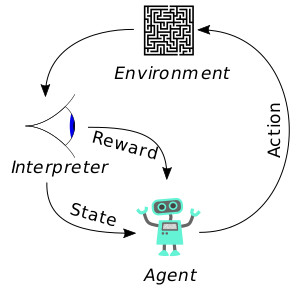
\includegraphics[width=.45\linewidth]{figures/01/rl.jpg}
    \caption{A typical reinforcement learning setup. The agent interacts with environment by performing actions, and receives reward and observation from interpreter as dictated by problem. Source: Wikipedia}
    \label{fig:01_rl}
\end{figure}

The goal of a reinforcement learning algorithm is to maximize the agent's total reward by repeatedly interacting with the environment. In the beginning, the RL agent knows nothing about the dynamics of the environment, but eventually learns to solve the problem by repeated trial and error. Therefore, reinforcement learning is general enough to be applied in a wide variety of problems from manufacturing \cite{01_manu}, to robot control \cite{01_control}, to finance \cite{01_finance}.  A detailed mathematical formulation of reinforcement learning problem is presented in Chapter \ref{chapter:background}.

\section{Deep Reinforcement Learning}
Today, most machine learning methods pose the learning problem as function learning from given data. Deep learning has been very successful in learning complex functions given enough data. In deep learning, the target function is represented by stacking multiple non-linear layers (a deep neural network) and the network parameters are optimized by gradient descending a problem-specific loss function. The deep neural networks have shown remarkable success in a variety of image recognition tasks \cite{01_imagenet}. 

\begin{figure}[htb]
    \centering
    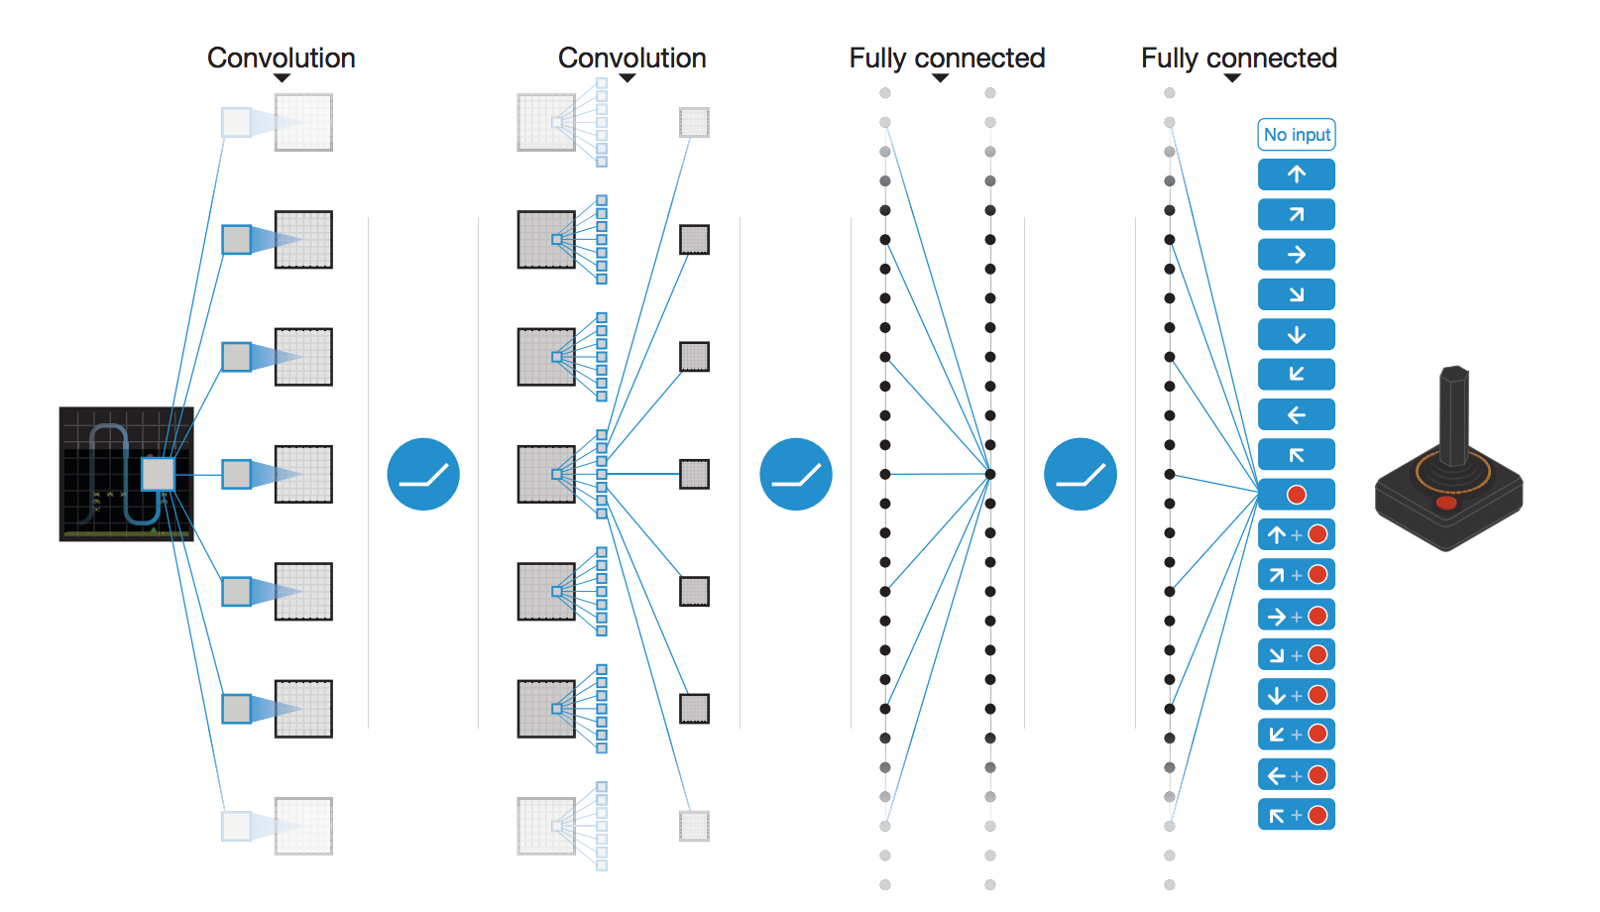
\includegraphics[width=.9\linewidth]{figures/01/dqn.png}
    \caption{The input to the network consists of 4 consecutive frames and it outputs Q-values for all possible actions. The action with highest Q-value is then chosen at this state. Source: \cite{mnih2015humanlevel}}.
    \label{fig:01_dqn}
\end{figure}

Deep reinforcement learning (DRL) is the study of reinforcement learning using deep neural networks as function approximators. Though neural networks have been used as function approximators in reinforcement learning for a long time, it recently got a lot of attention after the proposal of the deep Q-network algorithm (DQN) \cite{01_dqn}. DQN learns to play a wide range of Atari games from raw pixels and outperforms humans on some tasks. Recently, a new algorithm Alpha Go \cite{01_alphago} which also uses deep reinforcement learning, has learned to play Go better than human experts. 

Deep neural networks can be directly optimized to learn a mapping from inputs to outputs in supervised learning. However, applying deep neural networks in reinforcement learning problems is not that straightforward as there are many different choices where a function approximator can be used. For example, in case of Atari games, a neural network can be used either to predict the action to take at a particular state (pixel values) or to approximate the future expected reward for a state-action pair. DQN uses the latter formulation and approximates Q-values for all state-action pairs. The neural network used by DQN is illustrated in Figure \ref{fig:01_dqn}. The detailed classification of different deep reinforcement learning algorithms is given in Chapter \ref{chapter:related_work}.

\section{Stochastic Continuous Control}
Continuous control problems in reinforcement learning arise when the available actions of an agent are continuous valued. Continuous action spaces are usually more challenging than discrete action spaces \cite{ddpg}. A naive approach to modifying discrete action space algorithms, such as DQN, to continuous action domain would be to discretize the action space. However, this approach has several drawbacks. If the discretization is coarse, the output actions will not be smooth and will lead to unstable behavior. And if the discretization is fine, the number of discretized actions will be very high and intractable to learn. This situation becomes even worse as the number of different actions increases, due to the curse of dimensionality.

A \textit{policy} determines an RL agent's action selection process at a state. The policy can be either stochastic $\pi(a|s)$, the probability of an action $a$ given a state $s$ or deterministic $\pi(s)$, a deterministic mapping from state $s$ to action $a$. The stochastic policies are better than deterministic policies for many reasons. The randomness embedded in the stochastic policy lead to a better exploration of the state space which is important to learn a good policy. A stochastic policy is also required to calculate the policy gradients which are needed when policies are represented by neural networks.


\section{Contributions}

In this thesis, we consider continuous action space problems in deep reinforcement learning. We address the shortcomings of existing algorithms for stochastic continuous control and purpose a new formulation for such problems. Our proposed approach to making a policy stochastic is called Multiple Action Policy Gradients (MAPG). MAPG produces $M$ point estimates from the policy network at a state and then samples one action uniformly. The uniform random sampling from $M$ actions renders the resulting policy stochastic. 

The proposed formulation of the policy has several interesting implications. First, one can study the decision process of RL agent at runtime. A low variance among $M$ actions implies that the model only sees one way to act in a certain situation. A wider or even multi-modal distribution suggests that either there exist several possibilities given the current state or the model is unsure which action is the best. Second, the resulting stochastic policy by MAPG leads to a better exploration of the entire solution space and the final solution is of higher quality. Finally, MAPG can eliminate the external exploration mechanisms required during training e.g. Ornstein-Uhlenbeck process noise \cite{ounoise}, parameter noise \cite{paramnoise} or differential entropy of the normal distribution.

While MAPG helps in optimizing continuous policies, it has few drawbacks. It increases the overall training time of the algorithm. The value of $M$ is an hyper-parameter which needs to be tuned separately for different environments. 

In experiments, we evaluate MAPG on DDPG \cite{ddpg} algorithm on six continuous control problems of the OpenAI Gym \cite{greg2016} as well as a \textit{deep driving} scenario using the TORCS car simulator \cite{TORCS}. Then, we compare the performance of MAPG with DDPG \cite{ddpg}, A3C \cite{a3c} and SVG(0) \cite{svg} on all tasks. Further, we study the effects of MAPG on exploration during training and the quality of policy by analyzing the variance among different action values.
